\documentclass{report}

%* Packages Used

\usepackage[english]{babel}
\usepackage[utf8]{inputenc}

\usepackage{verbatim}
\usepackage{fancyvrb}

\usepackage{listings}
\usepackage{xcolor}


\usepackage{amsmath}
\usepackage{graphicx}
\usepackage{hyperref}
\usepackage{geometry}
\usepackage{float}


%* Package settings
\hypersetup{
colorlinks  = true,
linkcolor   = black,
urlcolor    = red,
}

\newgeometry{
      top = 0.75in,
      bottom = 0.75in,
      left = 0.75in,
      right = 0.75in,
}

\definecolor{codegreen}{rgb}{0,0.6,0}
\definecolor{codegray}{rgb}{0.5,0.5,0.5}
\definecolor{codepurple}{rgb}{0.58,0,0.82}
\definecolor{backcolour}{rgb}{0.95,0.95,0.92}
 
\lstdefinestyle{mystyle}{
    backgroundcolor=\color{backcolour},   
    commentstyle=\color{codegreen},
    keywordstyle=\color{magenta},
    numberstyle=\tiny\color{codegray},
    stringstyle=\color{codepurple},
    basicstyle=\footnotesize,
    breakatwhitespace=false,         
    breaklines=true,                 
    captionpos=b,                    
    keepspaces=true,                 
    numbers=left,                    
    numbersep=5pt,                  
    showspaces=false,                
    showstringspaces=false,
    showtabs=false,                  
    tabsize=2
}
\lstset{style=mystyle}
\lstset{language=Python}

%* Preamble
\title{

\includegraphics[width=0.5\textwidth]{resources/ua_logo.png} \\
Industrial Robotics TP2\\
\Large{University of Aveiro}
}

\author{Bruno Silva 98374\\
\href{https://github.com/brunofavs/TP2_RI}{Github Repository}
}

\setcounter{chapter}{1}

\begin{document}

\maketitle

\tableofcontents
\pagebreak


\section{Introduction}

This program was developed with the purpose of studying and consolidating
knowledge about robotic kinematics, including direct, inverse and differential
kinematics, three foundational pillars of any robotic system.

The general goal was to create an 9 degree of freedom(DOF) robot similar to a
construction crane, made of both rotational and prismatic joints, capable of
following a pre-determined path. The conceptual goal was to simulate the robot
that would be in a hypothetical real life scenario assembling big Christmas trees.

\begin{figure}[h]
    \centering
    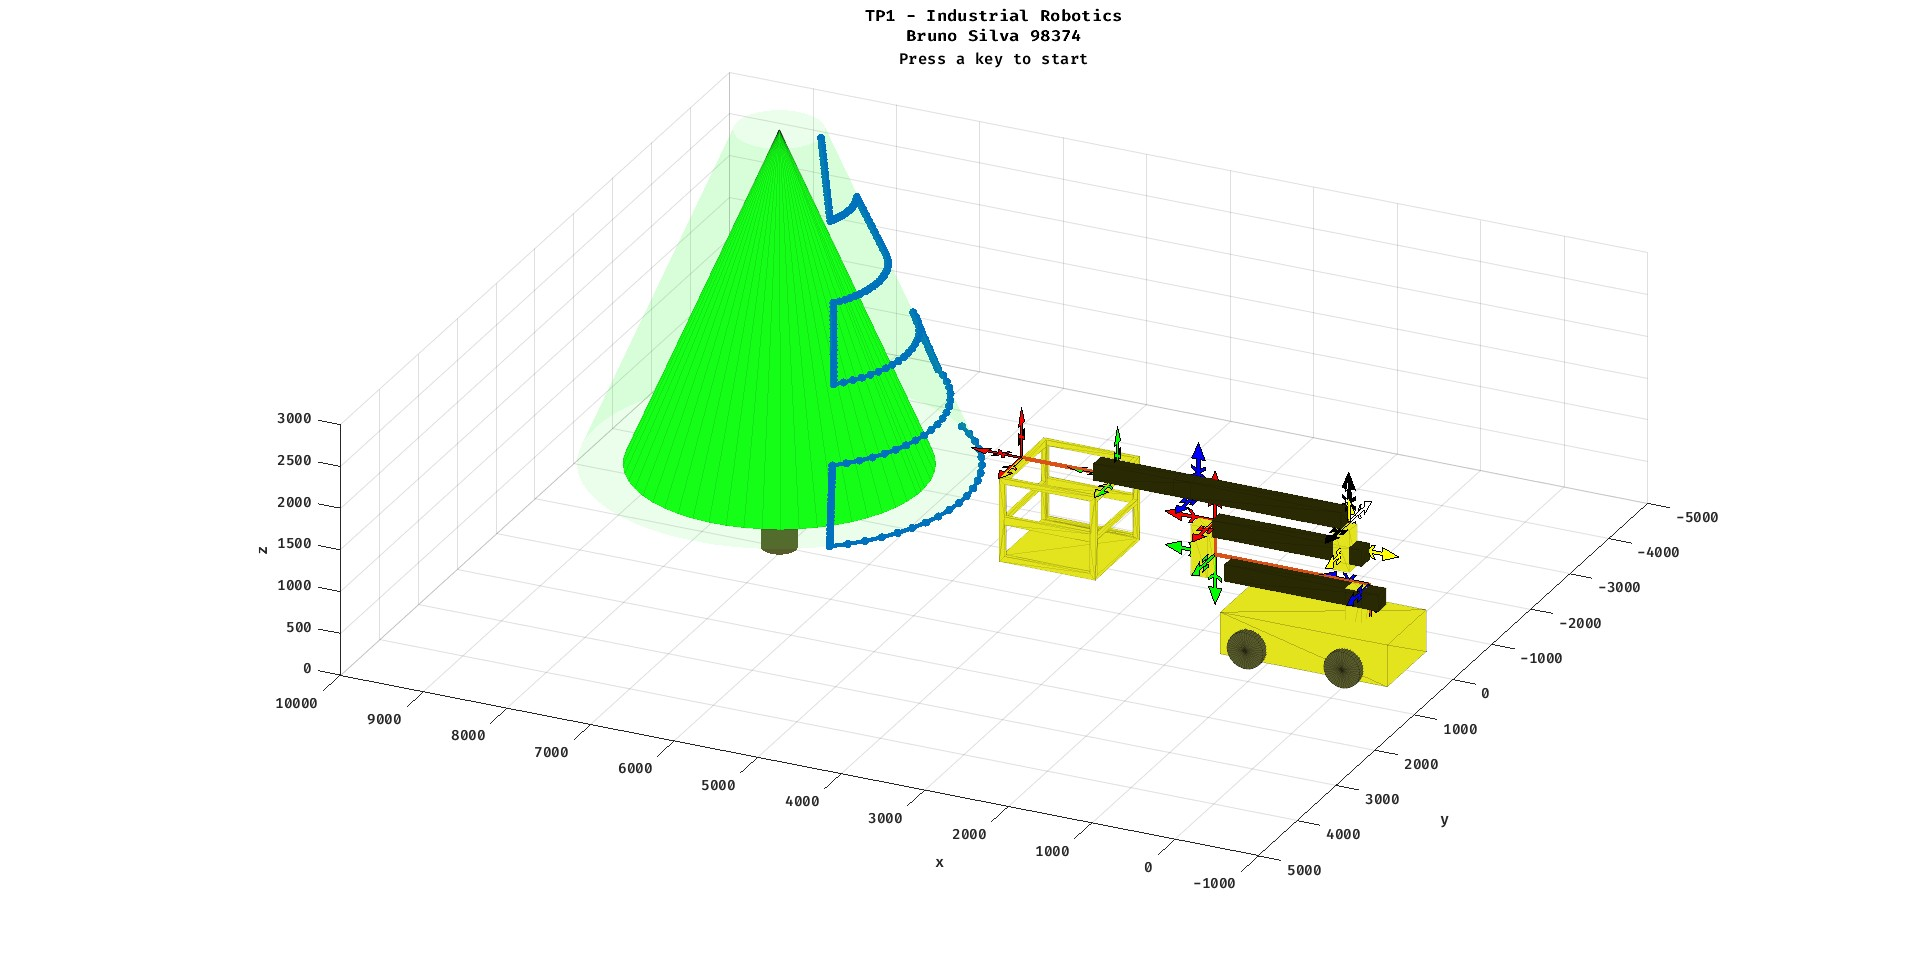
\includegraphics[scale=0.2]{resources/system_home.jpg}
    \caption{\label{fig:home}Robot and Path to follow.}
\end{figure}


\section{Script Analysis}

This section is aimed at briefly explaining the steps the script takes in order
to accomplish the desired objective as stated in the previous section.

\subsection{Tree Initialization}

The tree models were modeled in \textit{SolidWorks} and exported as
\textit{STL's}. Afterwards, a script found ind
\href{https://www.mathworks.com/matlabcentral/fileexchange/22409-stl-file-reader?s_tid=srchtitle}{\textit{Matlab's
File Exchange}} was used to import the \textit{STL's} into \textit{Matlab} as
patch objects. Being patch objects, any geometric transformation can be applied
to them. This was done to position the tree at the correct position and modify
the offset from the robot.

\subsection{Computing path and $\psi$}

If the tree had been drawn by computing the equations "by hand", this step
would've been easier. The procedure was the following:\begin{enumerate}
    \item Find the tip of the tree by visually inspecting the patch object drawn;
    \item Compute the end points of each segment based on the tree radius and height;
    \item Do linear interpolation for the linear segments
    \item Use the
    \href{https://www.mathworks.com/matlabcentral/fileexchange/123050-3d-arc-passing-through-3-points?s_tid=srchtitle}{\textbf{arc3}}
    to compute the point along the circular segments.\footnote{Unlike the first
    project, here the third point required by the script was quite easy to
    compute considering all circular segments are half full circles and were
    always on the \textit{Oxy} plane}
\end{enumerate}

To compute the angle of the tool end point (TCP) of the crane, a simple dot
product of the vectors made by the points represented in the \hyperref[fig:psi]{figure}.

\begin{figure}[h]
    \centering
    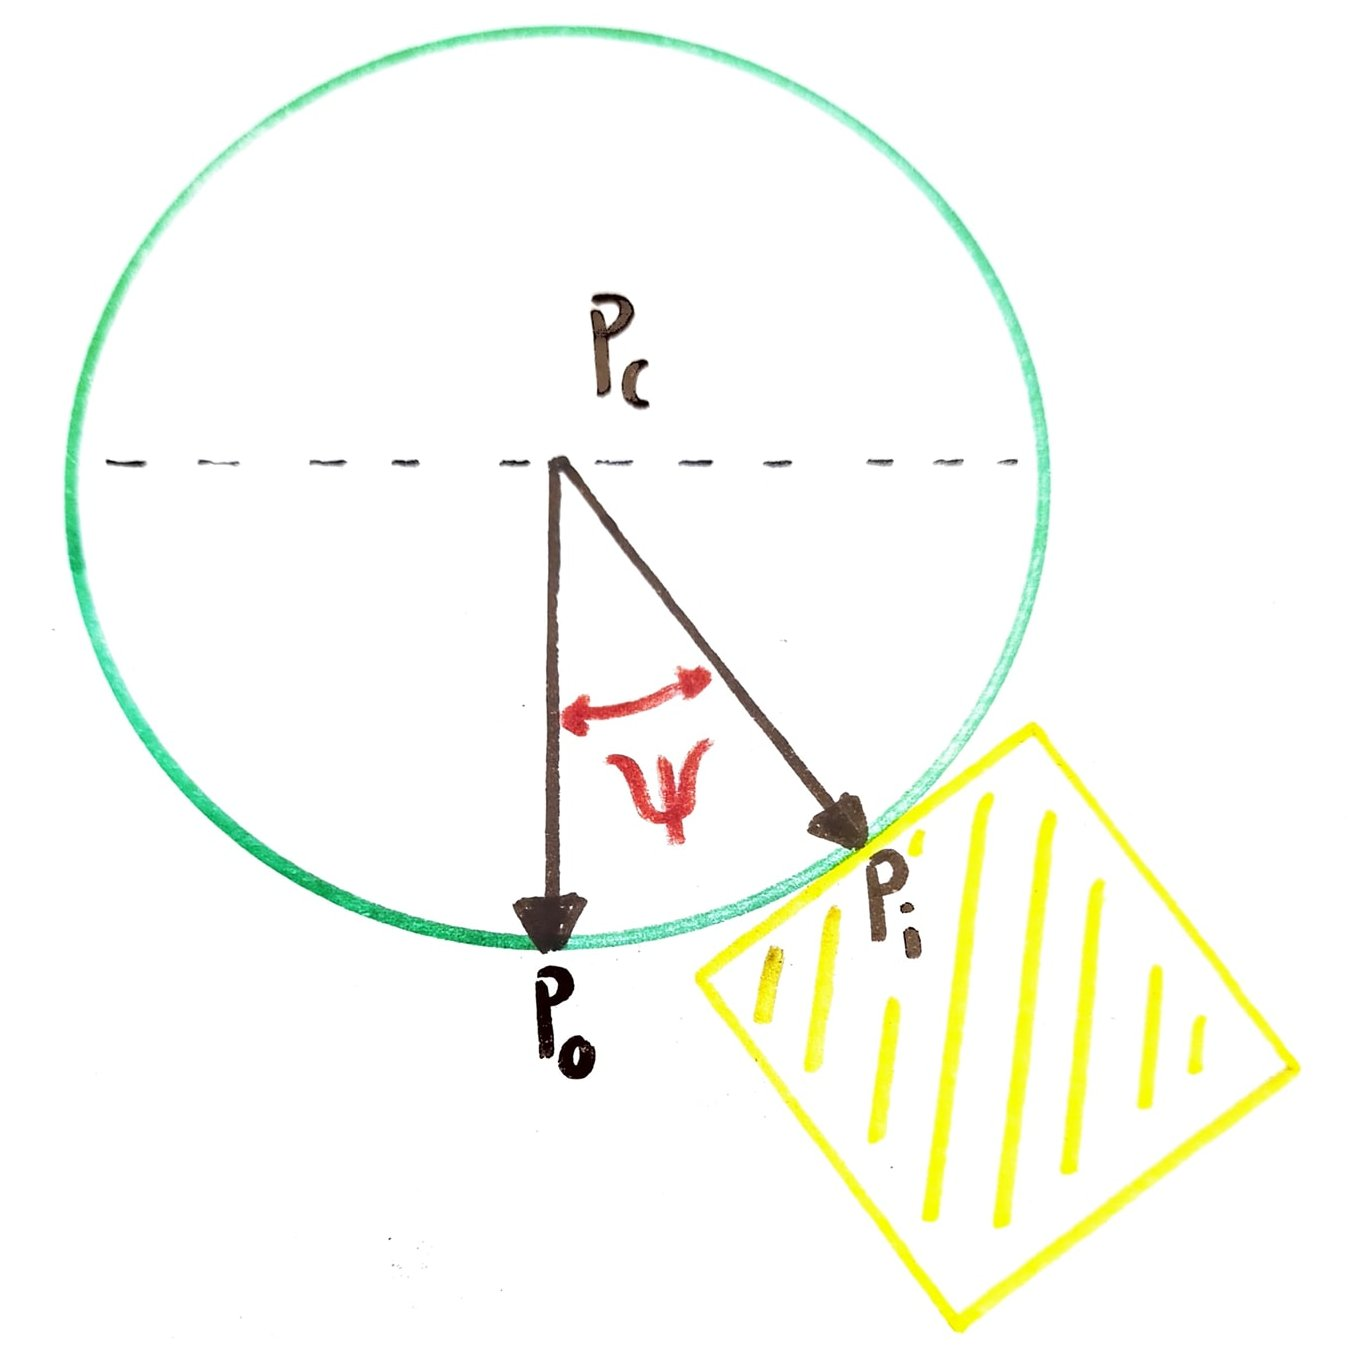
\includegraphics[scale=0.1]{resources/psi.jpeg}
    \caption{\label{fig:psi}$\psi$ computing based on a cross-section of the
    tree}
\footnote{The yellow square represents the operator's cabin}
\end{figure}

The \hyperref[fig:psi]{figure} represents a cross-section of the tree for a given radius.
Based on $P_c$,$P_0$,$P_i$, the angle $\psi$ is computed for each
point. Afterwards, to determine the angle signal, the cross-product of the same
vectors is computed.

\subsection{Robot Initialization}

The robot dimensions are loaded from a text file that should be present in the
main script's path and named \textit{"tp2.txt"}. The joint lengths should be in
the format $La = int$. A status message should be displayed to verify if the
parameters established by the user are correctly loaded.

In order to establish the \textit{\textbf{Denavit-Hartenberg}} parameters, a
schematic of the robot was made using a diagram drawing
software, \textit{LucidChart}. The reference frames and the resulting \hyperref[tab:dh]{\textbf{DH table}}
can be seen below:

\begin{figure}[h]
    \centering
    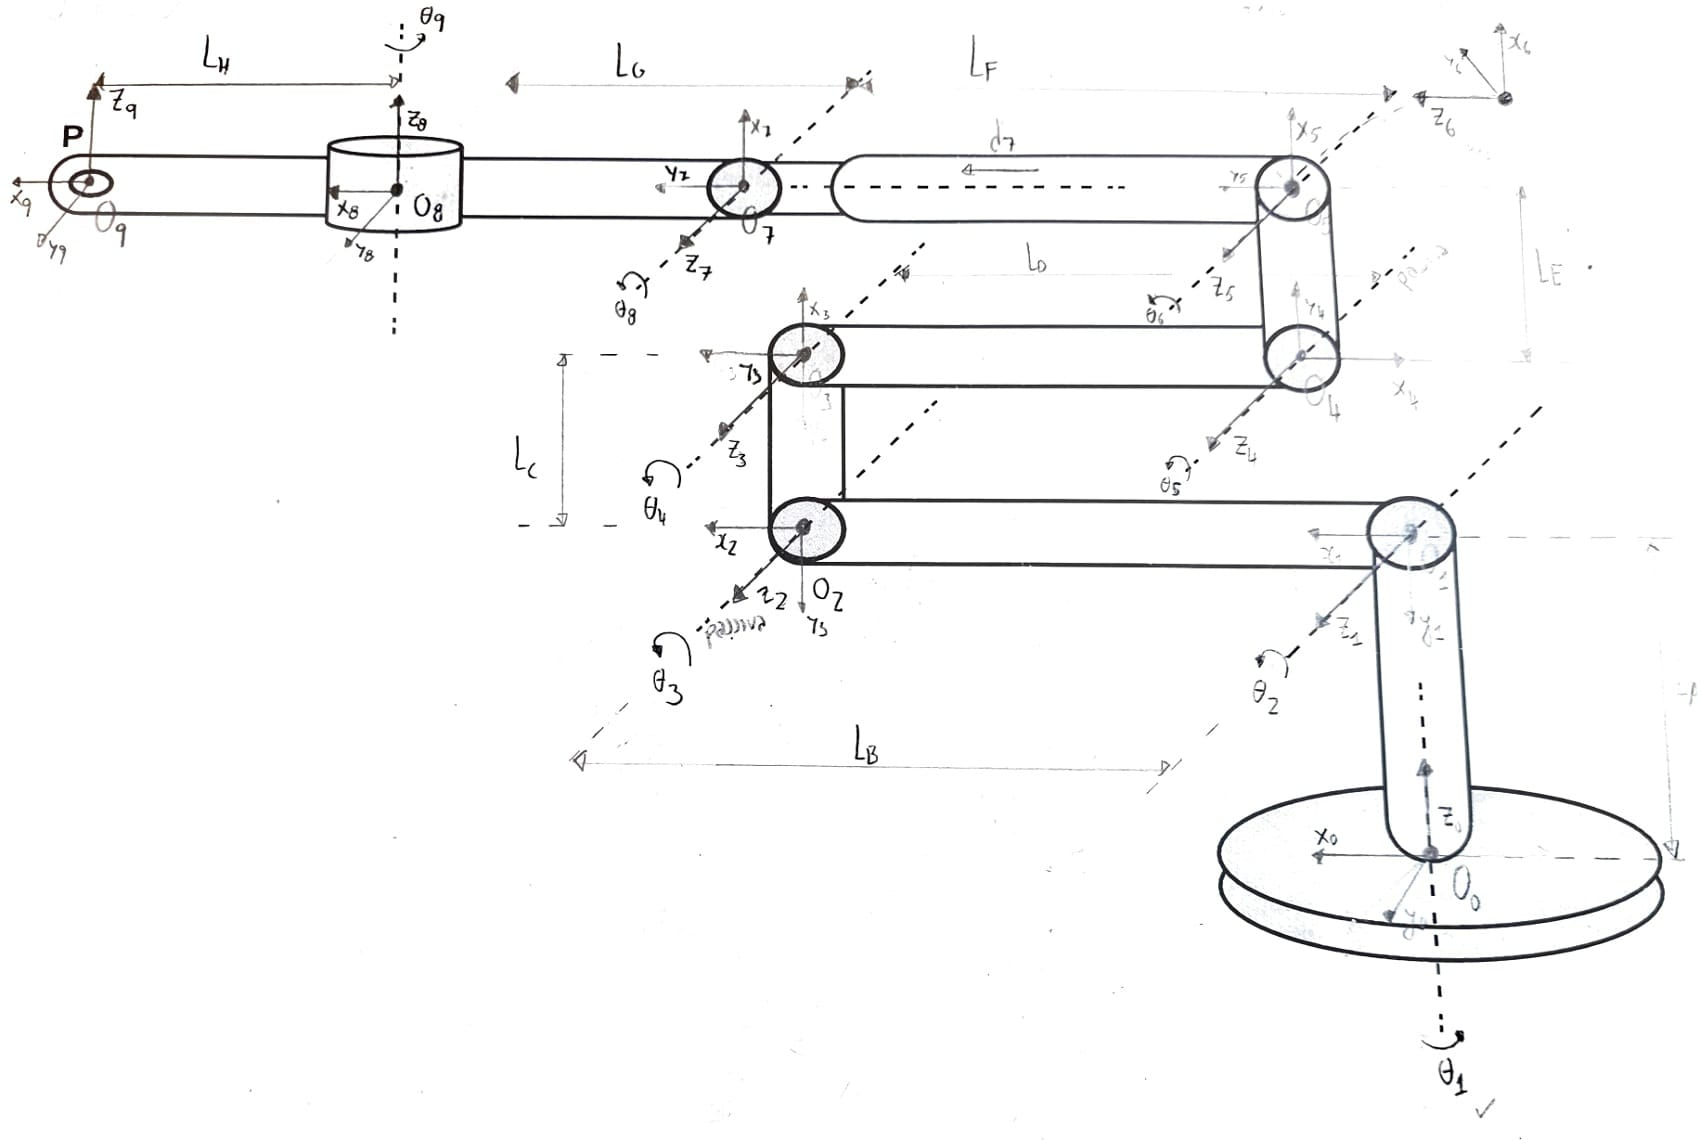
\includegraphics[scale=0.2]{resources/robot_draw.jpeg}
    \caption{\label{fig:r_draw}Robot schematic and reference frames}
\end{figure}

\begin{table}[H]
\centering
\begin{tabular}{|c|c|c|c|c|}
\hline
Joint & $\theta_i$ & $l_i$ & $d_i$ & $\alpha_i$ \\
\hline
1 & $\theta_1$ & 0 & $La$ & $-\frac{\pi}{2}$ \\
\hline
2 & $-\theta_2$ & $Lb$ & 0 & 0 \\
\hline
3 & $\theta_3 - \frac{\pi}{2}$ & $Lc$ & 0 & 0 \\
\hline
4 & $\theta_4 - \frac{\pi}{2}$ & $Ld$ & 0 & 0 \\
\hline
5 & $\theta_5 + \frac{\pi}{2}$ & $Le$ & 0 & 0 \\
\hline
6 & $\theta_6$ & 0 & 0 & $-\frac{\pi}{2}$ \\
\hline
7 & 0 & 0 & $Lf_{\text{min}} + d7$ & $\frac{\pi}{2}$ \\
\hline
8 & $\frac{\pi}{2} + \theta_8$ & $Lg$ & 0 & $\frac{\pi}{2}$ \\
\hline
9 & $\theta_9$ & $Lh$ & 0 & 0 \\
\hline
\end{tabular}
\caption{DH table}
\label{tab:dh}
\end{table}


To draw the joints, the same procedure used to load the trees was used. To align
them and move them with the robot reference frames, in the \textit{animateRobot}
function, the cumulative AA transformation was computed and was applied to each
body corresponding to the joint it was representing.

\subsection{Inverse Kinematics}

To compute the inverse kinematics(IK) the approach was the following: \begin{enumerate}
    \item Compute the IK of the joints 6 to 9;
    \item Compute the $\theta_1$ and update $\theta_9$ based on the $\psi$ angle;
    \item Compute the IK of the joints 2 to 6;
    \item Stitch the segments together.
\end{enumerate}

Matlab's symbolic calculus capabilities were heavily used to solve the equations
showed ahead.

The first segment, from joint 1 to 9, assumed that:\begin{itemize}
    \item $\theta_8 = -\theta_6$
\end{itemize}

With this simplification, the position elements of the AAA matrix from joint 6
to 9 yields the following system of equations :

\begin{equation}
\begin{cases}
    x_{69} = -\sin(\theta_6)(Lf_{\text{min}} + d7) \\
    y_{69} = Lg + Lf_{\text{min}}\cos(\theta_6) + Lh\cos(\theta_9) + d7\cos(\theta_6) \\
    z_{69} = Lh\sin(\theta_9)
\end{cases}
\end{equation}

Solving this system using Matlab's built-in solver gave the following results :

\begin{equation}
\begin{cases}
    q_9 = arcsin(\frac{z_{69}}{L_h})\\
    k = L_g + L_h*cos(q_9)-y_{69}\\
    q_6 = artan(\frac{x_{69}}{k})\\
    d_7 = \frac{sin(arctan(\frac{x_{69}}{k}))}{-L_{fMin}*sin(arctan(\frac{x}{k}))+x_{69}} 
\end{cases}
\end{equation}



\subsection{Differential Kinematics}

\subsection{Prismatic Joint Limit Analysis} 




\section{Additional notes}

\begin{itemize}

    \item Video links \begin{itemize}
        \item \href{}{Demo Video}
    \end{itemize}

    \item \href{https://github.com/brunofavs/TP2_RI}{Github Repository link}

\end{itemize}














\end{document}